%!TEX TS-program = xelatex
%!TEX encoding = UTF-8 Unicode
%!TEX root = 2020-GS-ARTICLE.tex
\newcommand{\mylanguages}{italian} % in reverse order
%-------------------------------------------------------------------------------
%-------------------------------------------------------------------------------
%	TITLE
%-------------------------------------------------------------------------------
%-------------------------------------------------------------------------------
\newcommand{\mytitle}{Corso di laurea in Musica Applicata}
\newcommand{\mysubtitle}{Corso di Sistemi, Tecnologie, Applicazioni e Linguaggi
di Programmazione\\
A.A. 2019-20}
%-------------------------------------------------------------------------------
%-------------------------------------------------------------------------------
%	AUTHORS
%-------------------------------------------------------------------------------
%-------------------------------------------------------------------------------
\newcommand{\authorone}{Davide Croci}
\newcommand{\institutione}{Conservatorio \emph{G. Nicolini} - Piacenza}
\newcommand{\emailone}{davide.croci@conservatorio.piacenza.it}
%-------------------------------------------------------------------------------
% \newcommand{\authortwo}{Wikio Orgopedio}
% \newcommand{\institutiontwo}{Conservatorio S. Cecilia di Roma}
% \newcommand{\emailtwo}{wikio @ orgopedio.com} % duplicate these 3 lines if more
%-------------------------------------------------------------------------------
%-------------------------------------------------------------------------------
%	PACKAGES AND OTHER DOCUMENT CONFIGURATIONS
%-------------------------------------------------------------------------------
%-------------------------------------------------------------------------------
\documentclass[
	a4paper,
	twocolumn
	]{article}
%--------------------------------------------------------------- GENERAL SETUP -
\usepackage[T1]{fontenc}
\usepackage[\mylanguages]{babel}
\usepackage{
  graphicx,
  dblfloatfix
}
\usepackage{graphicx}
\usepackage{epstopdf}
\epstopdfsetup{update}
\usepackage[usenames]{color}
\usepackage{amssymb}
\usepackage{hyperref} % For hyperlinks in the PDF
%---------------------------------------------------------------- STYLE GS2020 -
%!TEX TS-program = xelatex
%!TEX encoding = UTF-8 Unicode
%!TEX root = 2020-GS-ARTICLE.tex
%-------------------------------------------------------------------------------
%-------------------------------------------------------------------------------
%	CUSTOM PACKAGES AND OTHER DOCUMENT CONFIGURATIONS
%-------------------------------------------------------------------------------
%-------------------------------------------------------------------------------
\usepackage{Alegreya}
\linespread{1.05}
\usepackage{
	fontspec,
	xltxtra,
	xunicode
	}

\usepackage{
	xfrac,
	unicode-math
	}

\defaultfontfeatures{Mapping=tex-text}
\setmonofont[
	Scale=MatchLowercase
	]{Andale Mono}
\setmathfont[
	Scale=MatchLowercase,
	Scale=1
	]{Libertinus Math}

\usepackage{microtype}
\usepackage[
	top=20mm,
	bottom=25mm,
	textwidth=17.2cm,
	columnsep=0.8cm
	]{geometry}
\usepackage[
	hang,
	small,
	labelfont=bf,
	up,
	textfont=it,
	up
	]{caption}
\usepackage{paralist} % For compact item lists
\usepackage{etoolbox} % Some tools: used for quote environment
\AtBeginEnvironment{quote}{\small}
\usepackage{titling} % Customizing the title section
\usepackage{booktabs} % Horizontal rules in tables
\usepackage{enumitem} % Customized lists
\setlist[itemize]{noitemsep} % Make itemize lists more compact
\usepackage{abstract} % Allows abstract customization
\renewcommand{\abstractnamefont}{\normalfont\bfseries} % Set the "Abstract" text to bold
\renewcommand{\abstracttextfont}{\normalfont\small\itshape} % Set the abstract itself to small italic text
\usepackage{titlesec} % Allows customization of titles
\renewcommand\thesection{\Roman{section}} % Roman numerals for the sections
\renewcommand\thesubsection{\Roman{subsection}} % roman numerals for subsections
\titleformat{\section}[block]{\large\centering\bfseries}{\thesection.}{1em}{} % Change the look of the section titles
\titleformat{\subsection}[block]{\large}{\thesubsection.}{1em}{} % Change the look of the section titles
%-------------------------------------------------------------------------------
%-------------------------------------------------------------------------------
%	TITLE SECTION
%-------------------------------------------------------------------------------
%-------------------------------------------------------------------------------
\setlength{\droptitle}{-4\baselineskip} % Move the title up
\pretitle{\begin{center}\huge\bfseries} % Article title formatting
\posttitle{\end{center}} % Article title closing formatting
\title{\mytitle \\ \large{\emph{\mysubtitle}}} % Article title
\author{%
\textsc{\authorone}\\%
\normalsize \institutione \\ %
\normalsize \emailone %
% \and % duplicate these 4 lines if more
% \textsc{\authortwo} \\%
% \normalsize \institutiontwo \\ %
% \normalsize \emailtwo %
}
\date{} % Leave empty to omit a date

\usepackage{fancyhdr} % Headers and footers
\pagestyle{fancy} % All pages have headers and footers
\fancyhead{} % Blank out the default header
\fancyfoot{} % Blank out the default footer
\fancyhead[C]{\small \mytitle • \mysubtitle} % Custom header text
\fancyfoot[RO,LE]{\small \today~ • w: \input{includes/words.txt} • c: \input{includes/char.txt} • p:~\thepage} % Custom footer text
%-------------------------------------------------------------------------------
%-------------------------------------------------------------------------------
%	LISTINGS
%-------------------------------------------------------------------------------
%-------------------------------------------------------------------------------
\usepackage{listings}
% lstlistings setup
\definecolor{yobg}{rgb}{0.9,0.9,1}
\definecolor{yotxt}{rgb}{0.01,0.01,0.52} % a dark blue.
\definecolor{mylstbg}{rgb}{0.98,0.98,0.98} % a really pale grey.
\definecolor{mylstcmt}{rgb}{0.01,0.52,0.01} % a dark green.
\definecolor{mylstdoc}{rgb}{0.80,0.30,0.80} % a medium pink.

\lstset{%
  aboveskip=10pt,
	belowskip=5pt,
  language=C++,
  numbers=none,%left,%none,
  tabsize=4,
  %frame=single,
  breaklines=true,
  numberstyle=\tiny\ttfamily,
  backgroundcolor=\color{mylstbg},
  basicstyle=\footnotesize\ttfamily,
  commentstyle=\slshape\color{mylstcmt}, %\itshape,
  %frameround=tttt,
  columns=flexible, %fixed,
  showstringspaces=false,
  emptylines=2,
  inputencoding=utf8,
  extendedchars=true,
  literate=	{á}{{\'a}}1
			{à}{{\`a}}1
			{ä}{{\"a}}1
			{â}{{\^a}}1
			{é}{{\'e}}1
			{è}{{\`e}}1
			{ë}{{\"e}}1
			{ê}{{\^e}}1
			{ï}{{\"i}}1
			{î}{{\^i}}1
			{ö}{{\"o}}1
			{ô}{{\^o}}1
			{è}{{\`e}}1
			{ù}{{\`u}}1
			{û}{{\^u}}1
			{ç}{{\c{c}}}1
			{Ç}{{\c{C}}}1,
  emph={component, declare, environment, import, library, process},
  emph={[2]ffunction, fconstant, fvariable},
  emph={[3]button, checkbox, vslider, hslider, nentry, vgroup, hgroup, tgroup, vbargraph, hbargraph, attach},
  emphstyle=\color{yotxt}, %\underline, %\bfseries,
  morecomment=[s][\color{mylstdoc}]{<mdoc>}{</mdoc>},
  rulecolor=\color{black}
}

\usepackage[framemethod=tikz]{mdframed} % Allows defining custom boxed/framed environments

%-------------------------------------------------------------------------------
%--------------------------------------------------- INFORMATION ENVIRONMENT ---
%-------------------------------------------------------------------------------

% Usage:
% \begin{info}[optional title, defaults to "Info:"]
% 	contents
% 	\end{info}

\mdfdefinestyle{info}{%
	topline=false, bottomline=false,
	leftline=false, rightline=false,
	nobreak,
	singleextra={%
		\fill[black](P-|O)circle[radius=0.4em];
		\node at(P-|O){\color{white}\scriptsize\bf i};
		\draw[very thick](P-|O)++(0,-0.8em)--(O);%--(O-|P);
	}
}

% Define a custom environment for information
\newenvironment{info}[1][Info:]{ % Set the default title to "Info:"
	\medskip
	\begin{mdframed}[style=info]
		\noindent{\textbf{#1}}
}{
	\end{mdframed}
}

%-------------------------------------------------------------------------------
%----------------------------------------------------- BIOGRAFIA ENVIRONMENT ---
%-------------------------------------------------------------------------------

% Usage:
% \begin{bio}[optional title, defaults to "Info:"]
% 	contents
% 	\end{bio}

\mdfdefinestyle{bio}{%
	topline=false, bottomline=false,
	leftline=false, rightline=false,
	nobreak,
	singleextra={%
		\fill[black](P-|O)circle[radius=0.4em];
		\node at(P-|O){\color{white}\scriptsize\bf b};
		\draw[very thick](P-|O)++(0,-0.8em)--(O);%--(O-|P);
	}
}

% Define a custom environment for information
\newenvironment{bio}[1][Biografia:]{ % Set the default title to "Info:"
	\medskip
	\begin{mdframed}[style=bio]
		\noindent{\textbf{#1}}
}{
	\end{mdframed}
}

%-------------------------------------------------------------------------------
%------------------------------------------------------- WARNING ENVIRONMENT ---
%-------------------------------------------------------------------------------

% Usage:
% \begin{warn}[optional title, defaults to "Warning:"]
%	Contents
% \end{warn}

\mdfdefinestyle{warning}{
	topline=false, bottomline=false,
	leftline=false, rightline=false,
	nobreak,
	singleextra={%
		\draw(P-|O)++(-0.5em,0)node(tmp1){};
		\draw(P-|O)++(0.5em,0)node(tmp2){};
		\fill[black,rotate around={45:(P-|O)}](tmp1)rectangle(tmp2);
		\node at(P-|O){\color{white}\scriptsize\bf !};
		\draw[very thick](P-|O)++(0,-1em)--(O);%--(O-|P);
	}
}

% Define a custom environment for warning text
\newenvironment{warn}[1][Warning:]{ % Set the default warning to "Warning:"
	\medskip
	\begin{mdframed}[style=warning]
		\noindent{\textbf{#1}}
}{
	\end{mdframed}
}

%-------------------------------------------------------------------- ABSTRACT -
\renewcommand{\maketitlehookd}{%
\begin{abstract}
\noindent\input{includes/abstract.txt}
\end{abstract}
}
%-------------------------------------------------------------------------------
%-------------------------------------------------------------------------------
%	BEGIN DOCUMENT
%-------------------------------------------------------------------------------
%-------------------------------------------------------------------------------
\begin{document}
\maketitle
\thispagestyle{empty}
%-------------------------------------------------------------------------------
%-------------------------------------------------------------------------------
\section*{INTRODUZIONE}

L’obiettivo del corso era la creazione di un sintetizzatore virtuale accessibile
online, ma utilizzabile anche offline. In aggiunta l'idea di approfondire nuove
possibilità di analisi sonora e il poter mettere in pratica programmando
attraverso un linguaggio algebrico molto economico nozioni teoriche apprese
in altri corsi si è rivelata, almeno per quel che riguarda il
sottoscritto, uno stimolo aggiuntivo all'apprendimento di nuove nozioni. Il
pensiero iniziale era quello di partire da un modello proposto, poi
trasformatosi in proposta di resa modulare con utilizzo di singoli moduli
preesistenti. Il limite dei corsisti, essendo iscritti ad un corso di Musica
Applicata e non di Musica Elettronica pura, è la quasi totale assenza di
background per quanto riguarda i linguaggi di programmazione, e l'appoggiarsi a
modelli di riferimento già esistenti era necessaria e si è rivelata una mossa
vincente.
Alla fine il risultato ha preso il nome di "Superstereo Synth", e la metodologia
scelta per la sua realizzazione è stata la programmazione in linguaggio Faust
\cite{faust}. La tecnologia individuata è una sintesi sottrattiva modulata
da phaser.
%con opzione di utilizzo su varie piattaforme, sia tramite sito web che su
%diverse piattaforme, in modo che fosse

\section*{DESCRIZIONE INTERFACCIA GRAFICA}

\noindent Modulo di generazione sonora:

\begin{compactitem}
  \item switch saw/noise per selezione forma d’onda di partenza
  \item knob \emph{Fcut} per requenza di taglio normalizzata $0/1$
  \item knob \emph{Q} per determinare la larghezza di banda $0.7/25$
  \item knob \emph{Gain} $-96/+12$
\end{compactitem}

\bigskip

\noindent Modulo di phasing:

\begin{compactitem}
  \item switch \emph{Bypass} per attivare/disattivare l’effetto
  \item knob \emph{Lfo} per frequenza dell’onda modulante $0/16$
  \item knob \emph{Feedback} per retroazione con coefficienti $-1/1$
  \item knob \emph{Delay} degli allpass $1/100$
\end{compactitem}

\bigskip

\noindent Modulo master:

\begin{compactitem}
  \item knob \emph{Pan L-R} $-45/+45$
  \item slider \emph{Volume} (in dB) $-70/0$
  \item switch \emph{Mute} on/off
  \item n.2 meters per visualizzazione livello di uscita Left e Right
\end{compactitem}

\section*{DESCRIZIONE DEI PROCESSI AUDIO}

Il processo di elaborazione audio viene quindi ad essere, come già accennato,
una sintesi sottrattiva modulata da phaser e con un modulo di gestione di base
dell'uscita del segnale (Pan, Volume, Mute, Meters)

\begin{figure}[h]
\begin{center}
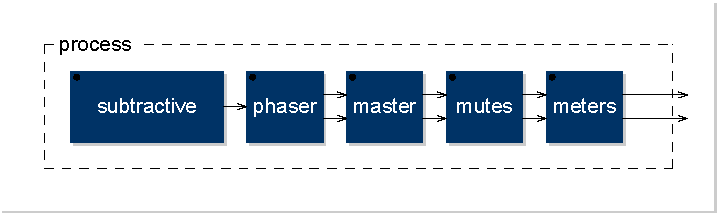
\includegraphics[width=.47\textwidth]{img/process.pdf}
\caption{\textbf{Process}. Struttura generale del sintetizzatore.}
\label{process}
\end{center}
\end{figure}

\subsection*{Sintesi sottrattiva saw/noise}

E’ un modello di sintesi nella quale una sorgente sonora, ricca di armoniche
(parziali), viene ad essere modificata da un punto di vista spettrale,
sottraendo opportunamente da essa bande di frequenze o singole parziali. La
sintesi sottrattiva altera il bilanciamento spettrale di un segnale: questa
tecnica dà i migliori risultati quando viene applicata a segnali dotati di uno
spettro molto ricco di armoniche, come quelli prodotti da generatori di rumore
o di impulsi. Questo procedimento è il più utilizzato per la produzione di
timbri nell'elettronica analogica, tanto che molti effetti tipici della sintesi
sottrattiva sono diventati sinonimo stesso di musica elettronica. Il principio
su cui si basa questa sintesi è quello di un generatore di forme
d'onda che abbiano già una propria conformazione armonica: un generatore di
rumore produce uno spettro distribuito a larga banda, un generatore di impulsi
produce invece una forma d’onda periodica ad una frequenza specifica che
possiede una grande quantità di energia nelle sue armoniche. In questo caso
tramite uno switch abbiamo la possibilità di scegliere tra un’onda saw (dente
di sega) e un generatore di rumore grigio.
Gli aspetti più interessanti della sintesi sottrattiva vengono evidenziati
attraverso un processo dinamico, ovvero quando questa operazione di filtraggio
si sviluppa durante l’evoluzione temporale del segnale.

\subsection*{Filtro, frequenza di taglio}

Il filtro scelto per operare sul suono del generatore è della tipologia
\emph{passa basso},ispirato al filtro Ladder di Bob Moog, ovvero un sistema che
permette il passaggio di frequenze al di sotto di una certa soglia, detta
frequenza di taglio (qui Fcut); un filtro modifica quindi l’ampiezza e la fase
di un segnale che passi attraverso di esso, senza alterare la frequenza di
alcuna componente spettrale del segnale stesso.
Tramite un filtro, quindi, vengono selezionate soltanto alcune delle componenti
di queste forme d'onda e le altre vengono escluse. Nell'analogico il
procedimento è abbastanza semplice; l'uscita dell'oscillatore viene inviata
all'ingresso di un filtro che in base alla frequenza di taglio seleziona una
determinata gamma di frequenze. Applicando un generatore di funzioni al filtro
otterremo una variazione continua delle frequenze selezionate. Questo
procedimento, molto empirico, ha il pregio di creare una variazione continua
dello spettro, cosa che è alla base della creazione dei suoni "sintetici".
La frequenza di taglio è definita come la frequenza alla quale l’energia
trasmessa dal filtro diminuisce di metà (-3 dB) rispetto alla massima energia
trasmessa dalla banda passante. Essendo un filtro di tipo digitale, la Fc o
Fcut è data dalla media aritmetica della frequenza di taglio superiore ed
inferiore.

\subsection*{Fattore di merito Q}

E' un parametro di smorzamento di un'oscillazione, ed è detto fattore di merito
o di qualità perchè misura la qualità desiderata in un circuito accordato o in
un risonatore.

\subsection*{Gain}

Con il gain ovviamente andiamo a definire il volume di partenza della forma
d’onda.

\subsection*{Modulo di phasing}

Il phasing è un processo modulativo che parte duplicando una forma d'onda di
partenza, ottenendo due segnali identici per intensità, frequenza e fase,
quindi un segnale doppio; nel caso in cui la fase di uno dei due segnali sia
invertita, si ha la cosiddetta controfase, in cui la somma dei segnali dà zero.
L'effetto di phaser si ottiene duplicando il segnale originale e ritardando
leggermente la copia; sommando le due forme d'onda si ottiene un effetto di
rotazione dovuto al fatto che i due segnali si trovano a volte in fase e a
volte fuori fase; questo effetto, denominato "phase shifter" è alla base del
funzionamento del phaser. Qui è usato un filtro all-pass, che, contrariamente
agli altri filtri, non elimina frequenze ma varia la fase del segnale audio
modificando le relazioni di fase tra le varie frequenze, secondo il modello di
Curtis Roads \cite{cr96cmt}.

\begin{figure}[h]
\begin{center}
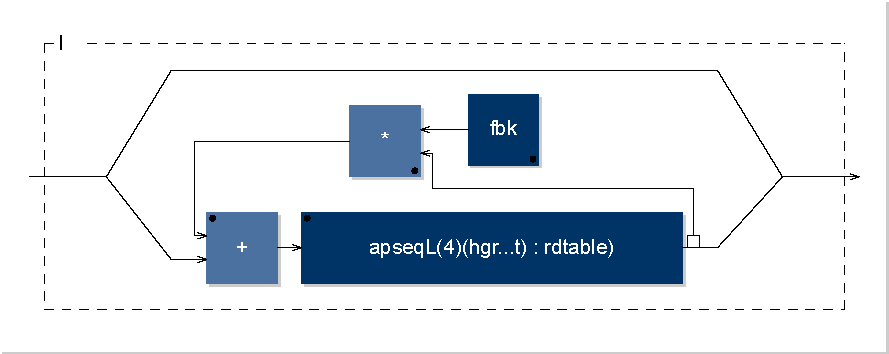
\includegraphics[width=.47\textwidth]{img/phaser.pdf}
\caption{\textbf{Phaser}.}
\label{phas}
\end{center}
\end{figure}

\subsection*{Bypass}

E' un pulsante che ovviamente permette di bypassare l'effetto per avere un
ascolto depurato dall'effetto phaser.

\subsection*{Lfo}

Sigla di Low Frequency oscillator, è un generatore di forme d'onda a frequenza
infrasonica, con funzione di modulatore d'effetti. In questo caso serve a
modulare l'effetto per poi sommarlo al segnale originale.

\subsection*{Feedback}

Determina la quantità di suono "filtrato" (ovvero cambiato di fase e
ritardato nel tempo) che ritorna al filtro stesso per essere ritardato
nuovamente; in pratica aumenta l'effetto uditivo del phaser rendendolo
molto più evidente.

\subsection*{Delay}

Regola lo sfasamento temporale della fase opposta alla forma d'onda originale.

%\vfill\null

\section*{DESCRIZIONE DEL CODICE}

Il codice si apre con una serie di dichiarazioni (comando declare) su nome app,
breve descrizione e autori.

\begin{lstlisting}
declare name "Superstereo Synth";
declare description "Subtractive Phaser Modulated Synth";
declare author "Davide Croci";
declare author "Giuseppe Messineo";
declare author "Gianmarco Romiti";
import("stdfaust.lib");
\end{lstlisting}

Segue la sezione GUI, in cui vengono definiti l'interfaccia grafica e tutti gli
elementi che la compongono (faders, knob, pulsanti...) e, nel caso dei master,
visualizzati con due faders, anche il range che li definisce (da -70 a 0 dB).

\begin{lstlisting}
// GUI
main(x) = hgroup("[01] Superstereo Synth",x);
s_g(x) = main(vgroup("[01] SUBTRACTIVE",x));
m_g(x) = main(vgroup("[03] MASTER",x));
p_g(x) = main(vgroup("[05] PHASER",x));
lmeter(x) = main(attach(x,an.amp_follower(0.150,x):ba.linear2db:vbargraph("[02]
			L [unit:dB]", -70,0)));
rmeter(x) = main(attach(x,an.amp_follower(0.150,x):ba.linear2db:vbargraph("[04]
			R [unit:dB]", -70,0)));
meters = lmeter, rmeter;
\end{lstlisting}

La sezione SUBTRACTIVE definisce le caratteristiche del segnale di partenza.
Viene fornita un'alternativa tra onda a dente di sega (saw) e rumore bianco
(noise) con un pulsante; successivamente mediante 3 knob si può controllare il
filtro di taglio, la larghezza di banda Q e il gain.

\begin{lstlisting}
// SUBTRACTIVE
// Sawfreq Custom
sawfreq = 123;
generator = (no.noise *switch),(os.sawtooth(sawfreq)*(1-switch)) :> _;
switch = s_g(checkbox("[01] Saw/Noise")) : si.smoo;
gain = s_g(vslider("[04] Gain [style:knob]",-12,-96,+12,0.01)) : ba.db2linear
			: si.smoo;
Q = s_g(vslider("[03] Q [style:knob]",5,0.7072,25,0.01));
fcut = s_g( vslider("[02] Cut [style:knob]",0.65,0,1,0.001)) : si.smoo;
subtractive = generator : ve.moogLadder(fcut,Q) : *(gain);
\end{lstlisting}

La sezione PHASER definisce i parametri dell'effetto phaser: un pulsante bypass,
e 3 knob per controllare Lfo, Feedback e Delay. Più avanti si stabilisce anche
la sequenza di N filtri all-pass di cui è composto, secondo il modello di Curtis
Roads \cite{cr96cmt}, un limiter (processore dinamico progettato per imoedire di
oltrepassare un dato livello di segnale ed evitare la distorsione) e un filtro
chopper che taglia drasticamente il segnale per evitare ridondanze derivate
dalla sovrapposizione delle fasi.

\begin{lstlisting}
// PHASER
lff = p_g(vslider("[02] Lfo [style:knob]", 0.358, 0, 16, 0.001)) : si.smoo;
fbk = p_g(vslider("[03] Feedback [style:knob]", -0.689, -0.999, 0.999, 0.001)
			: si.smoo);
del = p_g(nentry("[04] Delay [style:knob]", 1, 1, 100, 1));
lfo = os.osc(lff);
phaserLR(N,x,d,g,fb) = x <: l,r
with{
  allpassL(d,g) = (+ <: de.fdelay((ma.SR/2),d),*(-g)) ~ *(g) : mem,_ : +;
  allpassR(d,g) = (+ <: de.fdelay((ma.SR/2),d),*(g)) ~ *(-g) : mem,_ : +;
  apseqL(N,d,g) = seq(i,N,allpassL(d,g));
  apseqR(N,d,g) = seq(i,N,allpassR(d,g));

  l = _<: _, (+:apseqL(N,d,g))~*(fb):> _;
  r = _ <: _, (+:apseqR(N,d,g))~*(-fb):> _;
};

// N all-pass custom (min = sharp | max = smooth)
superstereophaser = phaserLR(4,_,del,lfo,fbk) : stereoshuffle;
// HARD LIMITER
chopper(a) = min(a) : max(-a);
// Chopper amp custom | Filter order custom | Filter freq custom
hardlimiter = chopper(0.7) : fi.lowpass(12,15000): chopper(0.9) :
			fi.lowpass6e(20000);
phchop = superstereophaser : hardlimiter, hardlimiter;
\end{lstlisting}

Sotto allo slider del MASTER è posizionato uno knob denominato WIDE per
controllare lo STEREO SHUFFLER (termine coniato da Alan Blumlein \cite{ab58} ),
ovvero l'apertura in stereo panning del segnale in uscita del synth; in pratica
un amplificatore della stereofonia.

\begin{figure}[h]%b=bottom,t=top, h=here
\begin{center}
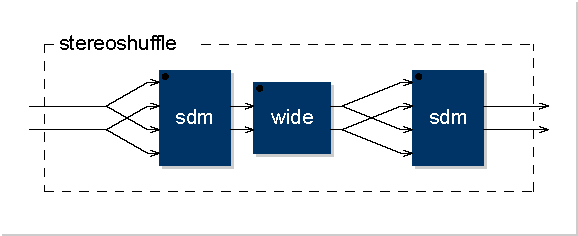
\includegraphics[width=.47\textwidth]{img/mid-side-shuffler.pdf}
\caption{\textbf{Stereo Shuffler}. descrizione.}
\label{shuff}
\end{center}
\end{figure}

\begin{lstlisting}
// STEREO SHUFFLER
pot = m_g(vslider("[02] WIDE [style:knob]",100,0,200,0.1)) : /(100) : si.smoo;
somma = + : /(2);
diff = - : /(2);
sdm = somma,diff;
wide = _, * (sqrt(pot));
stereoshuffle= _,_ <: sdm : wide <: sdm;
\end{lstlisting}

Infine la sezione MASTER CONTROLS permette di controllare i parametri di uscita
del suono: uno slider per definire il volume master di uscita, un pulsante Mute,
due meters per visualizzare anche a livello visivo l'andamento del suono in
uscita tra i due canali destro e sinistro.

\begin{lstlisting}
// MASTER CONTROLS
mute=m_g(*(1-(checkbox("[04] Mute")))) : si.smoo;
volume = m_g(vslider("[02] VOLUME ",-6,-70,12,0.1)) : ba.db2linear : si.smoo;
bpc = p_g(checkbox("[01] Bypass"));
phaser = ba.bypass1to2(bpc,phchop);
mutes = mute,mute;
master = (*(volume), *(volume));
process= subtractive : phaser : master : mutes : meters;
\end{lstlisting}

%\newpage % USE NEWPAGE TO FORCE COLUMNN INTERRUPTION
%-------------------------------------------------------------------------------
%-------------------------------------------------------------------------------
\section*{CONCLUSIONI}

Confrontarsi ex novo con i linguaggi macchina per creare un prodotto come questo
synth virtuale, pur nella sua semplicità, è interessante e ha dato spunti
interessanti per il futuro, chissà non diventi un punto di partenza per
sperimentare nuove possibilità sonore; sicuramente per il compositore
multimediale è un percorso imprescindibile, utile e ricco di sviluppi.
Un ultimo cenno sull'utilizzo dei programmi Atom, Latex e Github, prima
sconosciuti e che hanno permesso di redigere il presente in forma di
documento con una struttura di tipo e livello accademico, che senz'altro
verranno utilizzati per future pubblicazioni.

\begin{quote}
La musica è matematica, \\
ma la matematica non basta a spiegare la musica \\
(Tiziano Terzani) \cite{tizterz}.
\end{quote}
%
% \begin{table}[htp]
% \begin{center}
% \begin{tabular}{ll}
% \textbf{Stages} & \textbf{Dur.} \\
% \hline
% \textbf{Omnidirectional Expositions} & 6 mo. \\
% Sound-shape analysis and visualizations & \\
% Sound-shape reproduction & \\
% Sound-shape database design & \\
% \hline
% \textbf{Micro-Rhythm of sound-shape} & 12 mo. \\
% Solo repertoire analysis & \\
% Sound-shape explosion in practising & \\
% From literature to shapes open-data & \\
% \hline
% \textbf{Rhythm of sound-shape interactions} & 12 mo. \\
% Multiple sources multiple shapes & \\
% Relationship and complexity perception & \\
% \hline
% \textbf{Sound-shape in musical composition} & 12 mo. \\
% AI: unleashed writing opportunities & \\
% AI: can you listen the time? & \\
% \hline
% \textbf{Final documentation} & 6 mo. \\
% \end{tabular}
% \label{timesheet}
% \caption{Thinking Tetrahedral Today stages}
% \end{center}
% \end{table}%


%\begin{compactitem}
%\item Derivations of the Lorentz transformations
%\item Einstein–Hilbert action
%\item Tests of general relativity
%\item Two-body problem in general relativity
%\end{compactitem}


\vfill\null

\raggedright
\bibliographystyle{plain}
\bibliography{includes/bibliography.bib}

\end{document}

%%%%%%%%%%%%%%%%%%%%%%%%%%%%%%%%%%%%%%%%%%%%%%%%%%%%%%%%%%%%%%%%%%%%%%%%%%%%%%%%
% 2020 GIUSEPPE SILVI ARTICLE TEMPLATE BASED ON
%%%%%%%%%%%%%%%%%%%%%%%%%%%%%%%%%%%%%%%%%%%%%%%%%%%%%%%%%%%%%%%%%%%%%%%%%%%%%%%%
% Journal Article
% LaTeX Template
% Version 1.4 (15/5/16)
% This template has been downloaded from:
% http://www.LaTeXTemplates.com
% Original author:
% Frits Wenneker (http://www.howtotex.com) with extensive modifications by
% Vel (vel@LaTeXTemplates.com)
% License:
% CC BY-NC-SA 3.0 (http://creativecommons.org/licenses/by-nc-sa/3.0/)
%%%%%%%%%%%%%%%%%%%%%%%%%%%%%%%%%%%%%%%%%%%%%%%%%%%%%%%%%%%%%%%%%%%%%%%%%%%%%%%%
